%%%%%%%%%%%%%%%%%%%%%%%%%%%%%%%%%%%%%%%%%
% Beamer Presentation
% LaTeX Template
% Version 1.0 (10/11/12)
%
% This template has been downloaded from:
% http://www.LaTeXTemplates.com
%
% License:
% CC BY-NC-SA 3.0 (http://creativecommons.org/licenses/by-nc-sa/3.0/)
%
%%%%%%%%%%%%%%%%%%%%%%%%%%%%%%%%%%%%%%%%%

%----------------------------------------------------------------------------------------
%	PACKAGES AND THEMES
%----------------------------------------------------------------------------------------

\documentclass{beamer}

\mode<presentation> {

% The Beamer class comes with a number of default slide themes
% which change the colors and layouts of slides. Below this is a list
% of all the themes, uncomment each in turn to see what they look like.

%\usetheme{default}
%\usetheme{AnnArbor}
%\usetheme{Antibes}
%\usetheme{Bergen}
%\usetheme{Berkeley}
%\usetheme{Berlin}
%\usetheme{Boadilla}
%\usetheme{CambridgeUS}
%\usetheme{Copenhagen}
%\usetheme{Darmstadt}
%\usetheme{Dresden}
%\usetheme{Frankfurt}
%\usetheme{Goettingen}
%\usetheme{Hannover}
%\usetheme{Ilmenau}
%\usetheme{JuanLesPins}
%\usetheme{Luebeck}
\usetheme{Madrid}
%\usetheme{Malmoe}
%\usetheme{Marburg}
%\usetheme{Montpellier}
%\usetheme{PaloAlto}
%\usetheme{Pittsburgh}
%\usetheme{Rochester}
%\usetheme{Singapore}
%\usetheme{Szeged}
%\usetheme{Warsaw}

% As well as themes, the Beamer class has a number of color themes
% for any slide theme. Uncomment each of these in turn to see how it
% changes the colors of your current slide theme.

%\usecolortheme{albatross}
%\usecolortheme{beaver}
%\usecolortheme{beetle}
%\usecolortheme{crane}
%\usecolortheme{dolphin}
%\usecolortheme{dove}
%\usecolortheme{fly}
%\usecolortheme{lily}
%\usecolortheme{orchid}
%\usecolortheme{rose}
%\usecolortheme{seagull}
%\usecolortheme{seahorse}
%\usecolortheme{whale}
%\usecolortheme{wolverine}

%\setbeamertemplate{footline} % To remove the footer line in all slides uncomment this line
%\setbeamertemplate{footline}[page number] % To replace the footer line in all slides with a simple slide count uncomment this line

%\setbeamertemplate{navigation symbols}{} % To remove the navigation symbols from the bottom of all slides uncomment this line
}

\usepackage{graphicx} % Allows including images
\usepackage{booktabs} % Allows the use of \toprule, \midrule and \bottomrule in tables
\usepackage{amsmath}
\usepackage[english]{babel}
\usepackage{url,color}
\usepackage{subfigure}
\usepackage[export]{adjustbox}
\usepackage{amsthm,amsfonts,amssymb,amscd,amsxtra}
\usepackage{soul}
\usepackage{listings}
\usepackage{hyperref}

\usepackage{xcolor} % for setting colors
%----------------------------------------------------------------------------------------
%	TITLE PAGE
%----------------------------------------------------------------------------------------

\title[SIMD in C++]{SIMD in C++: auto-vectorization in a nutshell} 

\author{Anthony Boulmier} % Your name
\institute[UNIGE] % Your institution as it will appear on the bottom of every slide, may be shorthand to save space
{
Université de Genève \\
\medskip
\textit{anthony.boulmier@unige.ch} % Your email address
}
\date{\today} % Date, can be changed to a custom date

\newcommand{\R}{\mathbb{R}}
\newcommand{\x}{\textbf{x}}
\newcommand{\y}{\textbf{y}}
\renewcommand{\qedsymbol}{$\blacksquare$}
\newcommand{\dom}{\mathrm{dom}}
\newcommand{\ad}{\mathrm{ad}}
\newcommand{\gerado}{\mathrm{span}}
% set the default code style

\lstset{
    frame=tb, % draw a frame at the top and bottom of the code block
    tabsize=4, % tab space width
    showstringspaces=false, % don't mark spaces in strings
    numbers=left, % display line numbers on the left
    commentstyle=\color{green}, % comment color
    keywordstyle=\color{blue}, % keyword color
    stringstyle=\color{red} % string color
}

\begin{document}

%%%%%%%%%%%%
% Title
\begin{frame}
\titlepage 
\end{frame}

%%%%%%%%%%%%
% Outline
\begin{frame}
\frametitle{Outline}
\tableofcontents
\end{frame}

%%%%%%%%%%%%

\section{Introduction}

\frame{
	\frametitle{Motivation}
\begin{itemize}

\item<1-> CPU clock rate does not increase anymore
\item<2-> More cores $\rightarrow$ more transistors !
\item<3-> Or ? Do multiple instructions at the same time!
\begin{figure}
    
\includegraphics[width=3cm, center]{image/moores-law.jpg}
\end{figure}
\end{itemize}

}
%-------------------------------------------------%
\frame{
\frametitle{What is SIMD ?}
SIMD stands for: \textbf{S}ingle \textbf{I}nstruction \textbf{M}ultiple \textbf{D}ata 
\begin{itemize}
\item<1-> Same operation on multiple values (think about element-wise vector operations) 

Example: You want to sum the forces (XYZ) for 100K particles. Do $4$, $8$, or $16$ summations at the same time instead of $1$.

\item<2-> Recent CPUs have an instruction set that works on \textbf{vector registers} (\textit{\%xmm, \%ymm,} and \textit{\%zmm} registers, note: xmm are also used for scalar operations) 

\item<3-> Up to $16x$ performance improvement and it is almost free lunch !\\

Codes that benefit from vector instructions are called vectorized code.
\end{itemize}
}

\frame{
	\frametitle{Vector registers}
\begin{figure}
    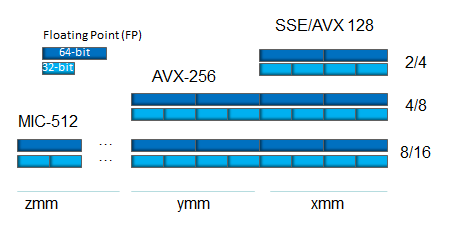
\includegraphics[width=10cm, center]{image/vector_registers.png}
    \caption{Vector registers, source: \href{run: https://cvw.cac.cornell.edu/mic/vector}{Cornell}}
    \label{fig:vecreg}
\end{figure}
}

\frame{
	\frametitle{What is SIMD ?}
\begin{figure}
    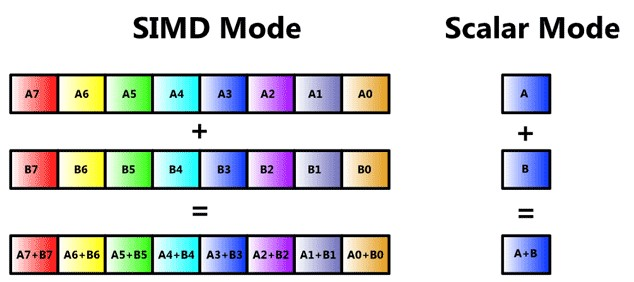
\includegraphics[width=10cm, center]{image/scalarvssimd.jpg}
    %\caption{Fugaku, 1st top500}
    \label{fig:fugaku}
\end{figure}
}

\frame{
	\frametitle{A LOT can be done with SIMD}
\begin{figure}
    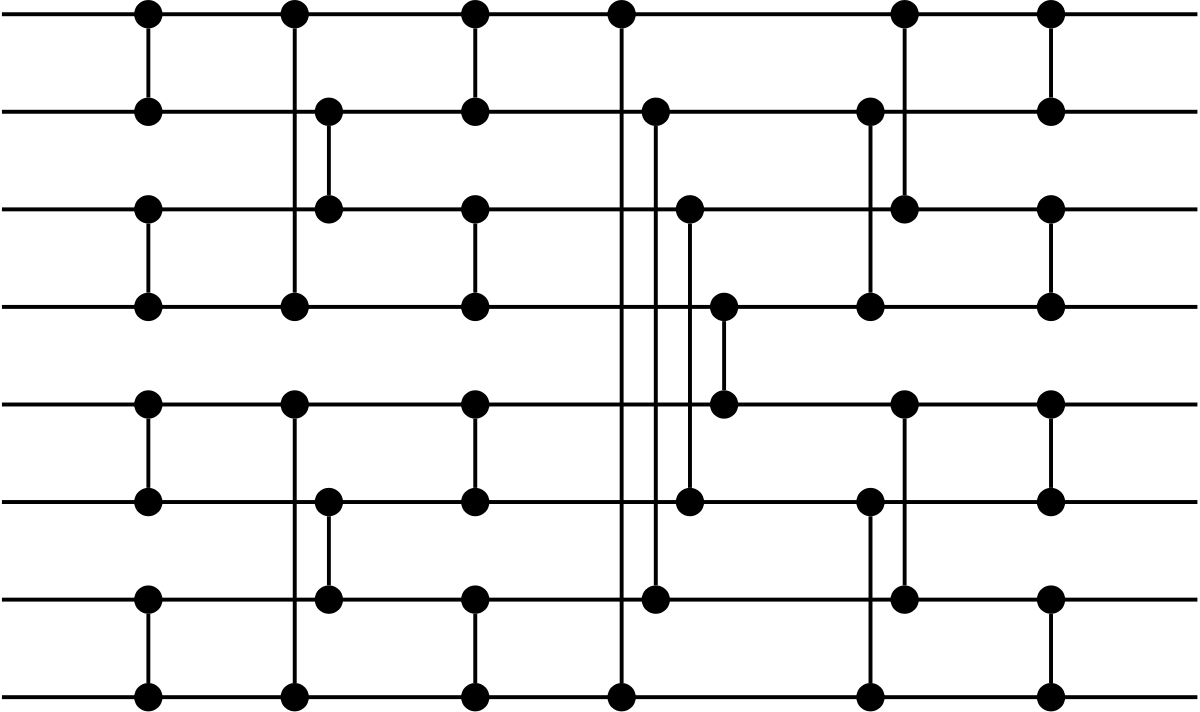
\includegraphics[width=10cm, center]{image/1200px-Batcher_Bitonic_Mergesort_for_eight_inputs.svg.png}
    \caption{What is this?}
    \label{fig:bitonicsort_simd}
\end{figure}
}
%-------------------------------------------------%

\section{How to ?}

\begin{frame}
\frametitle{How to write auto-vectorized code?}
Some portion of your codes may already benefits from it!

Compilers ``auto-vectorize'' under the following constraints:

\begin{itemize}
    \item<1-> Can only vectorize \text{for-loop} with a fixed (known at the beginning) number of iterations
    \item<2-> No dependency between array indices (iterations are independent)
    \item<3-> No conditional branching
    \item<4-> The compiler is sure that the performance will increase (use of cost function)
    \item<5-> Only vectorize inner loops\\
    \vspace{0.5cm}
    Rule of thumb: if you can't tell how to vectorize a code, neither can the compiler.
\end{itemize}
\end{frame}

%-------------------------------------------------%
\begin{frame}
\frametitle{Write and debug vectorized code}
\begin{enumerate}
    \item Write auto-vectorization friendly codes \\
    \textit{ Array of Structure (AoS) vs. Structure of Array (SoA) }
    
    \item Use the proper compilation line \\
    Vectorization is enabled by default at \textit{-O3}\\
    \textit{gcc -O2 -ftree-vectorize -fopt-info-vec-\{all,missed,optimized\} }\\
    \textit{clang -O2 -ftree-vectorize -Rpass-analysis=loop-vectorize -Rpass=loop-vectorize}
    
    \item Look at assembly code  \\
    \textit{-S -o main.s}
    
\end{enumerate}
\end{frame}
%-------------------------------------------------%
\begin{frame}[fragile]
\frametitle{Auto-vectorization friendly code}
\begin{block}{Example}
\begin{lstlisting}[language=C++, caption={AoS}]
const auto N = 100000;
struct Body {
    std::array<float, 2> v, p /*, ... */;
};
std::array<Body, N> bodies;
\end{lstlisting}
\end{block}
\end{frame}

\begin{frame}[fragile]
\begin{block}{Example}

\begin{lstlisting}[language=C++, caption={SoA}]
const auto N = 100000;
struct Bodies {
    std::array<float, N> vx, px, vy, py /*, ... */;
};
Bodies bodies;
\end{lstlisting}
\end{block}
\end{frame}

\begin{frame}{AoS}
    \begin{figure}
        \centering
        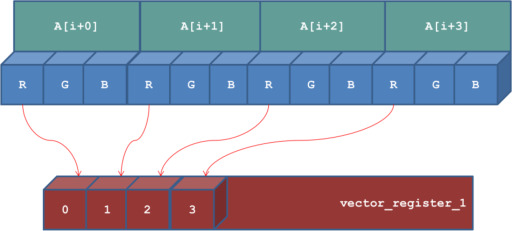
\includegraphics[width=10cm]{image/AoS.jpg}
        \caption{non-coalesced memory access, source: \href{run: https://www.sciencedirect.com/science/article/pii/B9780128091944000119}{Jeffers et al. 2016}}
        \label{fig:aos-memory}
    \end{figure}
\end{frame}
\section{Breaking the code!}

\begin{frame}[fragile]
\frametitle{Simple code}
\begin{block}{Example}
\begin{lstlisting}[language=C++, caption={Vectorization example}]
/* ... */
float f(float * a, float * b){
    #pragma GCC ivdep
    for(int i=0;i < 10000000; ++i)
      a[i] = a[i] + b[i];
    return a[50000];
}
/* ... */
\end{lstlisting}
\end{block}
\href{run:http://www.godbolt.org}{godbolt.org: online disassembler}
\end{frame}

\begin{frame}[fragile]
\frametitle{Simple code}
\begin{block}{Behind the scene (non-vectorized)}
\begin{lstlisting}[language=C++, caption={Vectorization example}]
.L2:
    movss   xmm0, DWORD PTR [rdi+rax]
    addss   xmm0, DWORD PTR [rsi+rax]
    movss   DWORD PTR [rdi+rax], xmm0
    add     rax, 4
    cmp     rax, 40000000
    jne     .L2
\end{lstlisting}

\end{block}
In godbolt.org: gcc-10 -O2
\end{frame}

\begin{frame}[fragile]
\frametitle{Simple code}
\begin{block}{Behind the scene (vectorized)}
\begin{lstlisting}[language=C++, caption={Vectorization example}]
.L2:
    vmovups zmm1, ZMMWORD PTR [rsi+rax]
    vaddps  zmm0, zmm1, ZMMWORD PTR [rdi+rax]
    vmovups ZMMWORD PTR [rdi+rax], zmm0
    add     rax, 64
    cmp     rax, 40000000
    jne     .L2
\end{lstlisting}
\end{block}
In godbolt.org: gcc-10 -O2 -ftree-vectorize -mavx512f\\
\pause
What if the array size in byte is not divisible by the vector register size? \\
\pause 
The compiler executes the rest in scalar mode.

\footnotesize{Note: unaligned calls are equivalent to aligned code since \textit{Intel Sandy Bridge}: see, \href{run: https://www.agner.org/optimize/instruction_tables.pdf}{Agner Fog}}
\end{frame}

\begin{frame}[fragile]
\frametitle{Exercise}
\begin{block}{What does the compiler say?}
\begin{lstlisting}[language=C++, caption={Vectorization example}]
void f(float* A, float* B, int N){
    for(int i = 0; i < N; ++i)
        A[i] = A[i] * B[i];
}
\end{lstlisting}
\end{block}
g++-10 main.cpp -O3 -mavx512f -fopt-info-vec-all -o main\\
\pause
\footnotesize \begin{lstlisting}[language=bash]
main.cpp:3:19: optimized: loop vectorized using 64 byte vectors
main.cpp:3:19: optimized:  loop versioned for vectorization 
because of possible aliasing
\end{lstlisting}
The compiler built a vectorized version, but it had to add aliasing checks
\end{frame}

\begin{frame}[fragile]
\frametitle{Exercise}
\begin{block}{What does the compiler say?}
\begin{lstlisting}[language=C++, caption={Vectorization example}]
void f(float* A, float* B, int N){
#pragma GCC ivdep
    for(int i = 0; i < N; ++i)
        A[i] = A[i] * B[i];
}
\end{lstlisting}
\end{block}
gcc-10 main.cpp -O3 -mavx512f -fopt-info-vec-all -o main\\
\pause
\footnotesize \begin{lstlisting}[language=bash]
main.cpp:3:19: optimized: loop vectorized using 64 byte vectors
\end{lstlisting}
Compiled to avx512 instruction set !
\end{frame}

\begin{frame}[fragile]
\frametitle{Simple code}
\begin{block}{What does the compiler say?}
\begin{lstlisting}[language=C++, caption={Vectorization example}]
float f(float* A, float* B, int N){
#pragma GCC ivdep
    for(int i = 1; i < N; ++i)
        A[i] = A[i-1] * B[i-1];
    return A[0];
}
\end{lstlisting}
\end{block}
gcc-10 main.cpp -O3 -mavx512f -fopt-info-vec-all -o main\\
\pause
\footnotesize \begin{lstlisting}[language=bash]
main.cpp:5:18: missed: could not vectorize loop
main.cpp:6:21: missed: not vectorized: no vectype 
for stmt:_8=*_7
\end{lstlisting}
\end{frame}

\begin{frame}[fragile]
\frametitle{Simple code}
\begin{block}{What does the compiler say?}
\begin{lstlisting}[language=C++, caption={Vectorization example}]
float f(float* A, float* B, int N){
#pragma GCC ivdep
    for(int i = 1; i < N; ++i)
        if(A[i] < 3) A[i] = A[i] * B[i];
    return A[0];
}
\end{lstlisting}
\end{block}
gcc-10 main.cpp -O3 -mavx512f -fopt-info-vec-all -o main\\
\pause
\footnotesize \begin{lstlisting}[language=bash]
main.cpp:5:18: missed: could not vectorize loop
main.cpp:5:18: missed: not vectorized: control flow in loop.
\end{lstlisting}
\end{frame}


\section{Benchmarks}

\begin{frame}{Benchmark description}
    \begin{itemize}
        \item Two arrays ($x$,$y$) containing $S = 10^7$ float (32 bits).
        \item Iterate over the arrays and execute a function that costs $X$ flops. The function is generated and inlined at compile time using \textit{constexpr}.
        \item Do this $T$ times and compute min, max, and average computing time in serial mode and (auto)vectorized mode.
        \item<2-> Function MULSUM: \\
        $f_{\text{MUL}}(X, x_i, y_i) = y_i * f_{\text{MUL}}(X-1, y_i, x_i)$\\
        $f_{\text{MUL}}(0, x_i, y_i) = y_i$\\
        Example: $f(2, x_i, y_i)=y_i*x_i*y_i$
        \item<3-> Function FMASUM:\\
        $f_{\text{FMA}}(X, x_i, y_i) = y_i + \sum_1^X x_iy_i$\\
        Example: $f_{\text{FMA}}(2, x_i, y_i)=y_i+x_iy_i + x_iy_i$\\
        Note: I consider \textit{fused multiply add (FMA)} to cost $1$ flop.
    \end{itemize}
\end{frame}

\begin{frame}{Benchmark}
\begin{figure}
    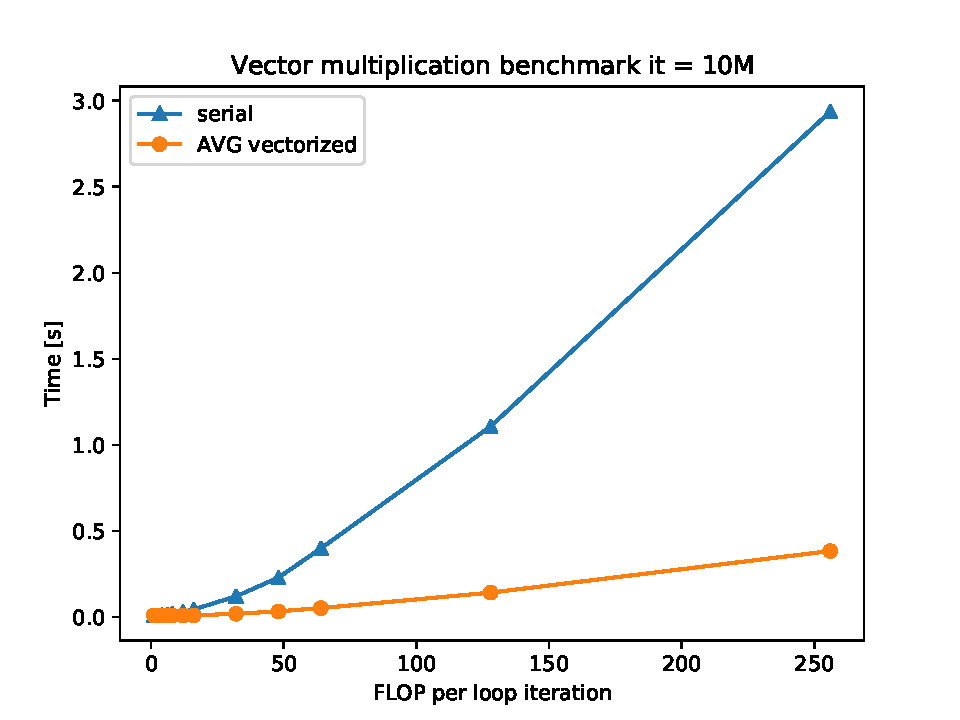
\includegraphics[width=9cm, center]{gcc/MUL/time_vec_vs_ser_vector_op.pdf}
    \caption{Time, gcc-10, Intel i7-10750H (Comet Lake): with avx2 (ymm 256 bits)}
    \label{fig:time}
\end{figure}
\end{frame}

\begin{frame}{Benchmark}
\begin{figure}
    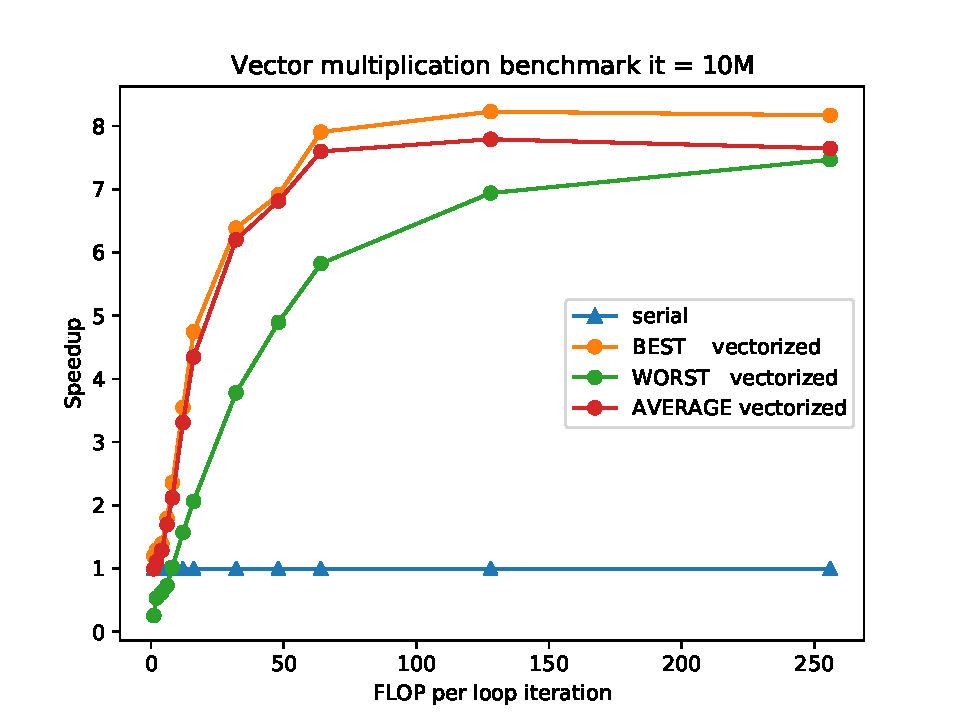
\includegraphics[width=9cm, center]{gcc/MUL/speedup_vec_vs_ser_vector_op.pdf}
    \caption{Speedup, gcc-10, Intel i7-10750H (Comet Lake): with avx2 (ymm 256 bits)}
    \label{fig:speedup}
\end{figure}
\end{frame}

\begin{frame}{Benchmark}
\begin{figure}
    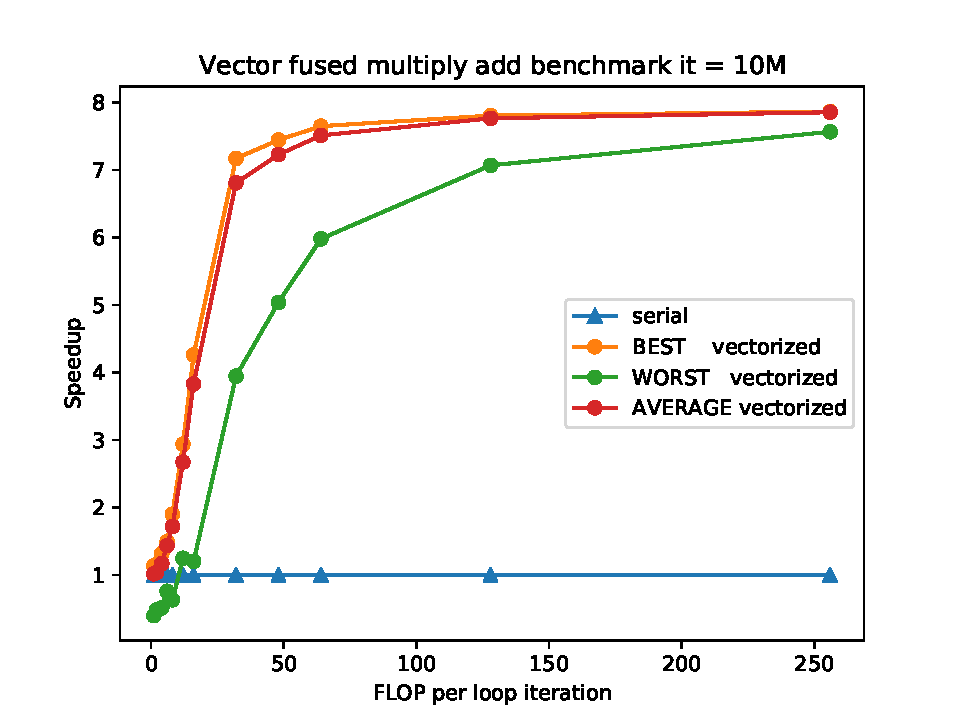
\includegraphics[width=9cm, center]{gcc/FMA/speedup_vec_vs_ser_vector_op.pdf}
    \caption{Speedup, gcc-10, Intel i7-10750H (Comet Lake): with avx2 (ymm 256 bits)}
    \label{fig:speedup}
\end{figure}
\end{frame}

\begin{frame}{clang 10: huho}
\begin{center}
        main.cpp:69:3: remark: the cost-model indicates that interleaving is not beneficial [-Rpass-analysis=loop-vectorize]
\end{center}
\end{frame}

\begin{frame}{Benchmark}
\begin{figure}
    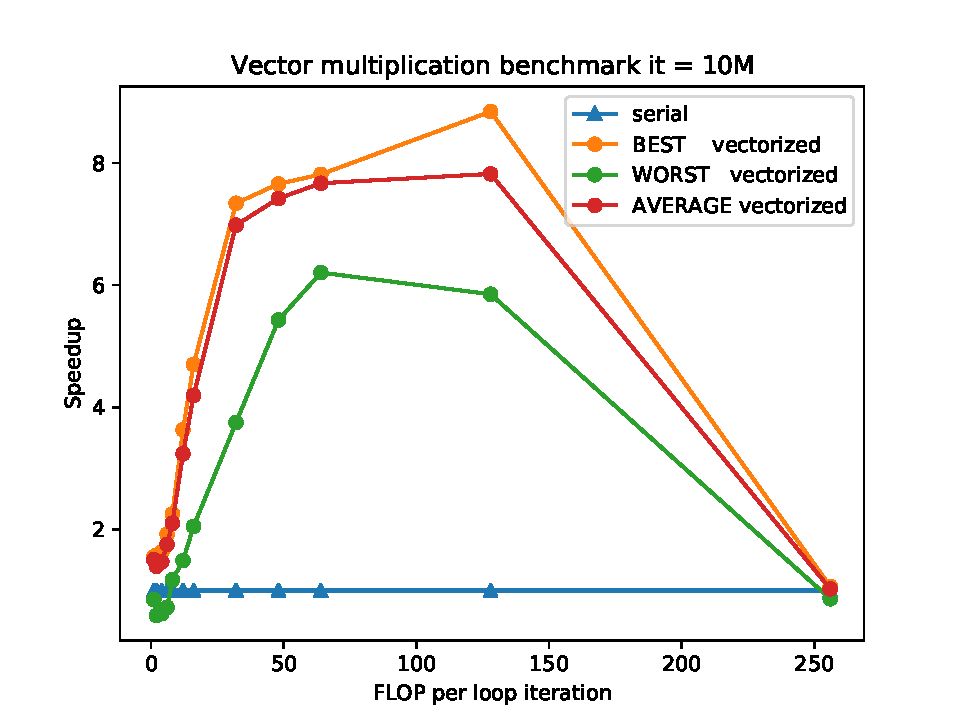
\includegraphics[width=9cm, center]{clang/speedup_vec_vs_ser_vector_op.pdf}
    \caption{Speedup, clang-10, Intel i7-10750H (Comet Lake): with avx2 (ymm 256 bits)}
    \label{fig:speedup}
\end{figure}
\end{frame}

\begin{frame}{Benchmark summary}
\begin{enumerate}
    \item<1-> Bad news 1: when there is a few FLOP per iteration, the computation is bounded by memory transfer. Push/Pull to/from vector registers can kill your perfs!
    \item<2-> Bad news 2: the compiler can mispredict performance and it may not vectorize, even straightforward code.
    \item<3-> Good news: you can still sometimes be $N$ times faster. $N=\frac{\text{register size}}{\text{type size}}$
\end{enumerate}
\end{frame}

\section{Conclusion}
\begin{frame}{Conclusion}
\begin{itemize}
    \item SIMD requires the proper data structure and fine-grained data parallelism 
    \item Using vector registers and auto-vectorization, this can increase performance of data-parallel loop by a factor 4, 8, 16
    \item The compiler can auto-vectorize under \textit{many} constraints, some code may be impossible to auto-vectorize
    \item The compiler can be wrong
    \item Debugging auto-vectorized code is \textbf{tedious}
    \item Be careful about the overhead for vectorization (push/pull to/from vector registers)
\end{itemize}

\end{frame}
\begin{frame}{Next talk}
    \begin{center}
        \Huge If you want something done right, you have to do it yourself!
    \end{center}
\end{frame}
\end{document}